\chapter{VaR and Credit Risk}\label{var-and-credit-risk---practical-lesson-9}

\subsection{Overview}\label{overview}

In past lessons we have already seen the concepts of credit event,
survival probability and hazard rate. Today we will concentrate more on
the credit risk topic studying few more examples.

\section{Value at Risk}\label{value-at-risk}

The value at risk (VaR) of a portfolio is a function of two parameters
(time horizon and confidence level) and it is usually involved when it
is important to know to a certain precentage of confidence (\(X\)) how
much will be the maximum loss in the next $N$ days. It can be
interpreted as the loss level over \(N\) days that has a probability of
only \((100 - X)\%\) of being exceeded.

Mathematically the VaR is the loss corresponding to the
\((100-X)\textrm{th}\) precentile of the distribution of the change in
the value of the portfolio over the next \(N\) days. For example, with
\(N=1\) and \(X=95\), VaR is the fifth percentile of the distribution of
changes in the value of the portfolio over the next day (e.g.~in the
next picture the graphical representation of the VaR assuming a normal
distribution for the changes of value, see Fig.~\ref{fig:var_loss}).

    \begin{figure}
    \centering
      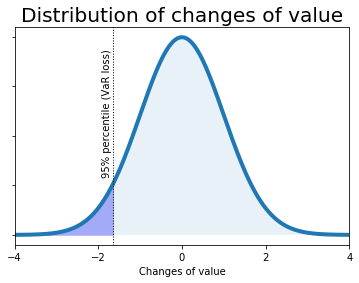
\includegraphics[width=0.6\linewidth]{lecture_9_files/lecture_9_2_0.png}
      \caption{Example of 5\% percentile on a Gaussian distribution.}
      \label{fig:var_loss}
    \end{figure}
    
    VaR is useful to summarize all the information about the risk of a
portfolio in one single number, but this can be also considered its main
limitation (too much simplification).

Concerning the time horizon parameter it is usually set to \(N=1\) since
it is not easy to estimate market variables over periods longer than 1
day. To generalize the VaR estimate it is assumed:

\[\textrm{N-day VaR} = \textrm{1-day VaR}\times \sqrt{N}\]

This relation is true only if the value changes of the portfolio over
the considered period of time have indipendent and identical normal
distributions with mean 0 (otherwise it is just an approximation).

\section{How to Estimate the VaR}\label{how-to-estimate-the-var}

\subsection{Historical Simulation}\label{historical-simulation}

In order to estimate the VaR from an historical series, we need to
collect the market variables affecting the portfolio over the last \(N\)
days (with \(N\) quite large).

The variation over each day in our time interval will provide different
scenarios to be applied to today's market simulation so that for each of
them we need to compute the variation in the portfolio value
(\(\Delta P\)). Our VaR estimate will be the (100 - X)\% percentile of
the resulting distribution. Given the 1-day VaR it is then possible to
determine the N-day VaR using the above formula.

Of course such historical simulation relies on the assumption that past
behaviors are indicative of what might happen in the future.

\subsubsection{Example:}\label{example}
Imagine a portfolio \(P\) whose value depends only on two market
variables (\(x_1(t) , x_2(t)\)). From the historical series of the
market variables we can determine various \emph{simulated} portfolio
values:

\[P_i(t_n+1) = P\Big(x_1(t_n)\frac{x_1(t_i)}{x_1(t_{i-1})} , x_2(t_n)\frac{x_2(t_i)}{x_2(t_{i-1})}\Big)\]

Essentially rescaling the market variables according to the variation
between day \(i\) and \(i-1\) we can draw a distribution of the possible
changes in the portfolio value \(P_i\) and then compute the VaR taking
the appropriate percentile.

    \begin{tcolorbox}[breakable, size=fbox, boxrule=1pt, pad at break*=1mm,colback=cellbackground, colframe=cellborder]
\begin{Verbatim}[commandchars=\\\{\}]
\PY{c+c1}{\PYZsh{} assuming the last value is today\PYZsq{}s one}
\PY{n}{var} \PY{o}{=} \PY{p}{[}\PY{l+m+mf}{0.56}\PY{p}{,} \PY{l+m+mf}{0.75}\PY{p}{,} \PY{l+m+mf}{0.44}\PY{p}{,} \PY{l+m+mf}{0.50}\PY{p}{]}

\PY{n}{scenario1} \PY{o}{=} \PY{n}{var}\PY{p}{[}\PY{o}{\PYZhy{}}\PY{l+m+mi}{1}\PY{p}{]} \PY{o}{*} \PY{n}{var}\PY{p}{[}\PY{l+m+mi}{1}\PY{p}{]} \PY{o}{/} \PY{n}{var}\PY{p}{[}\PY{l+m+mi}{0}\PY{p}{]}
\PY{n}{scenario2} \PY{o}{=} \PY{n}{var}\PY{p}{[}\PY{o}{\PYZhy{}}\PY{l+m+mi}{1}\PY{p}{]} \PY{o}{*} \PY{n}{var}\PY{p}{[}\PY{l+m+mi}{2}\PY{p}{]} \PY{o}{/} \PY{n}{var}\PY{p}{[}\PY{l+m+mi}{1}\PY{p}{]}
\PY{n}{scenario3} \PY{o}{=} \PY{n}{var}\PY{p}{[}\PY{o}{\PYZhy{}}\PY{l+m+mi}{1}\PY{p}{]} \PY{o}{*} \PY{n}{var}\PY{p}{[}\PY{l+m+mi}{3}\PY{p}{]} \PY{o}{/} \PY{n}{var}\PY{p}{[}\PY{l+m+mi}{2}\PY{p}{]}
\end{Verbatim}
\end{tcolorbox}

\subsection{How to Compute Percentiles in Python}\label{how-to-compute-percentiles-in-python}

Although later we will see how to compute percentiles of a gaussian distribution
without using python but for I would like to mention that \texttt{numpy}
has a convenient functions to compute n-percentiles of a generic
distribution:

    \begin{tcolorbox}[breakable, size=fbox, boxrule=1pt, pad at break*=1mm,colback=cellbackground, colframe=cellborder]
\begin{Verbatim}[commandchars=\\\{\}]
\PY{k+kn}{import} \PY{n+nn}{numpy}

\PY{n}{dist} \PY{o}{=} \PY{p}{[}\PY{l+m+mi}{1}\PY{p}{,} \PY{l+m+mi}{2}\PY{p}{,} \PY{l+m+mi}{3}\PY{p}{,} \PY{l+m+mi}{4}\PY{p}{,} \PY{l+m+mi}{5}\PY{p}{,} \PY{l+m+mi}{6}\PY{p}{,} \PY{l+m+mi}{7}\PY{p}{,} \PY{l+m+mi}{8}\PY{p}{,} \PY{l+m+mi}{9}\PY{p}{]}
\PY{n}{perc} \PY{o}{=} \PY{n}{numpy}\PY{o}{.}\PY{n}{percentile}\PY{p}{(}\PY{n}{dist}\PY{p}{,} \PY{p}{[}\PY{l+m+mi}{1}\PY{p}{,} \PY{l+m+mi}{50}\PY{p}{]}\PY{p}{)}
\PY{n+nb}{print} \PY{p}{(}\PY{n}{perc}\PY{p}{)}

[1.08 5.  ]
    \end{Verbatim}
\end{tcolorbox}

    \begin{tcolorbox}[breakable, size=fbox, boxrule=1pt, pad at break*=1mm,colback=cellbackground, colframe=cellborder]
\begin{Verbatim}[commandchars=\\\{\}]
\PY{c+c1}{\PYZsh{} when dealing with gaussian distributions a couple more of}
\PY{c+c1}{\PYZsh{} functions may be useful}
\PY{c+c1}{\PYZsh{} all of them refers to a standard gaussian mu=0; sigma=1}
\PY{k+kn}{from} \PY{n+nn}{scipy}\PY{n+nn}{.}\PY{n+nn}{stats} \PY{k}{import} \PY{n}{norm}

\PY{n+nb}{print} \PY{p}{(}\PY{n}{norm}\PY{o}{.}\PY{n}{pdf}\PY{p}{(}\PY{l+m+mi}{0}\PY{p}{)}\PY{p}{)}    \PY{c+c1}{\PYZsh{} value of gaussian for X=0}
\PY{n+nb}{print} \PY{p}{(}\PY{n}{norm}\PY{o}{.}\PY{n}{cdf}\PY{p}{(}\PY{l+m+mi}{0}\PY{p}{)}\PY{p}{)}    \PY{c+c1}{\PYZsh{} value of the integral from \PYZhy{}inf to 0}
\PY{n+nb}{print} \PY{p}{(}\PY{n}{norm}\PY{o}{.}\PY{n}{ppf}\PY{p}{(}\PY{o}{.}\PY{l+m+mi}{01}\PY{p}{)}\PY{p}{)}  \PY{c+c1}{\PYZsh{} 1\PYZpc{} percentile of normal gaussian}

0.3989422804014327
0.5
-2.3263478740408408
    \end{Verbatim}
    \end{tcolorbox}

\subsection{Model Approach}\label{model-approach}

Imagine that a portfolio \(P\) consists of different amounts \(a_i\)
invested on various assets. If with \(\Delta x_i\) we denote the daily
return of the $i$th asset the change in the value of the portfolio can be
expressed as:

\[\Delta P = \sum_{i=1}^n a_i \Delta x_i\]

If we then assume that the asset variations are normally distributed
with mean 0 (in this approach is typical to assume the expected change
in a market variable over the considered period zero), \(\Delta P\) will
be normally distributed (as a sum of normal distribution) with zero
mean.

To estimate the VaR we just need to compute the standard deviation of
\(\Delta P\). In the general case with many different assets we define
\(\sigma_i\) the daily volatility of the $i$th asset and with
\(\rho_{ij}\) the correlation coefficient between the assets $i$ and $j$.
The variance of \(\Delta P\) can then be expressed as:

\begin{align*}\sigma^2_P & = \sum_{i=1}^{n}\sum_{j=1}^{n}\rho_{ij}a_i a_j \sigma_i \sigma_j \\
& = \sum_{i=1}^{n} a_i^2 \sigma_i^2 + 2 \sum_{i=1}^{n}\sum_{j<i}^{n}\rho_{ij}a_i a_j \sigma_i \sigma_j \end{align*}

As in the previous case if we are interested in a longer time horizon we
can use the previous relationship between 1-day VaR and N-day VaR.

\subsubsection{Transformation to Standard
Normal}\label{transformation-to-standard-normal}

Values of the Standard Normal Gaussian (\(Z = \mathcal{N}(0,1)\))
percentiles are tabled everywhere and from them it is possible to
derive the values relative to any other gaussian distributions.

Given a generic gaussian \(\mathcal{N}(\mu , \sigma)\), we can go back
to the standard gaussian as:

\[Z= \frac{X-\mu}{\sigma}\]

and from the table above get the correct percentile.

Assume you need to know the percentage of a generic gaussian
\(\mathcal{N}(\mu=20 ,\sigma=5)\) above \(X=30\):

\[Z=\frac{X-\mu}{\sigma} = \frac{30-20}{5}=2\]

So we just need to check on the table above the percentage related to
\(Z=2\) which is 2.28\% (look at row -2.00, colum .00). Thus, 2.28\% of
the population with a normal distribution
\(\mathcal{N}(\mu=20 ,\sigma=5)\) lies above \(X=30\):

\[P(X>30)=P(Z>2)=0.0228\]

Conversely if you need to know the 1\% percentile of a generic gaussian
\(\mathcal{N}(\mu=20 ,\sigma=5)\), first look for .01 in the table above
and check the corresponding \(Z\) value (-3.1). Finally inverting the
above formula get the right value of the percentile:

\[ X= \sigma Z + \mu = 5\cdot -3.1 + 20 = 4.5 \]

\subsection{Monte Carlo Simulation}\label{monte-carlo-simulation}

A very useful alternative to the previous approaches is using a Monte
Carlo simulation to generate the probability distribution for the
\(\Delta P\) distribution. Imagine we need to compute the 1-day VaR for
a portfolio, the following steps need to be implemented:

\begin{itemize}
\tightlist
\item
  determine today's value of the portfolio;
\item
  simulate the evolution of all the portfolio market variables in one
  day;
\item
  recompute the value of the portfolio using the simulated market
  variables;
\item
  compute the \(\Delta P\) value as the simulated minus today's value of
  the portfolio;
\item
  repeat from the second step on as many times as needed to build the
  probability distribution for \(\Delta P\).
\end{itemize}

VaR is finally estimated as the appropriate percentile of the
probability distribution of \(\Delta P\).

For a more detailed description of Monte Carlo simulation see Chapter~\ref{cap:montecarlo}.

\subsection{Stress Testing and Back
Testing}\label{stress-testing-and-back-testing}

In addition to calculating VaR, it can be useful to perform a
\emph{stress test}. This essentially implies to estimate how a portfolio
would behave under the most extreme market moves seen in the last 20
years. To test those effects from the historical series are taken the
market variables seen in a particular day with exceptional large
variations. The idea is to take into account extreme events that can
occur but that have such low probability that are hard to simulate
(e.g.~a 5-standard deviation move should happen once every 7000 years
but in practice can be observed twice over 10 years.

    \begin{tcolorbox}[breakable, size=fbox, boxrule=1pt, pad at break*=1mm,colback=cellbackground, colframe=cellborder]
\begin{Verbatim}[commandchars=\\\{\}]
\PY{c+c1}{\PYZsh{} how to compute how likely is a n\PYZhy{}sigma event ? }
\PY{c+c1}{\PYZsh{} (assuming gaussian dist.)}
\PY{c+c1}{\PYZsh{} the probability is the integral of the distribution}
\PY{c+c1}{\PYZsh{} from \PYZhy{}inf to n\PYZhy{}sigma}

\PY{k+kn}{from} \PY{n+nn}{scipy}\PY{n+nn}{.}\PY{n+nn}{stats} \PY{k}{import} \PY{n}{norm}
\PY{n}{prob} \PY{o}{=} \PY{n}{norm}\PY{o}{.}\PY{n}{cdf}\PY{p}{(}\PY{o}{\PYZhy{}}\PY{l+m+mi}{5}\PY{p}{)} \PY{o}{*} \PY{l+m+mi}{2} \PY{c+c1}{\PYZsh{} since I\PYZsq{}m fine with +\PYZhy{} 5sigma movements}
\PY{n}{nyears} \PY{o}{=} \PY{l+m+mi}{1}\PY{o}{/}\PY{n}{prob}\PY{o}{/}\PY{l+m+mi}{252}
\PY{n+nb}{print} \PY{p}{(}\PY{n}{nyears}\PY{p}{)}

6921.737673091067
    \end{Verbatim}
\end{tcolorbox}

    Another important check to be done is the so-called \emph{back testing}
which consists of checking how well the VaR estimate would have
performed in the past. Basically it has to be tested how often the daily
loss exceeded the N-days X\% VaR just computed. If it happens on about
(100-X)\% of the times we can be confident that our estimate is correct.

\section{Credit Ratings}\label{credit-ratings}

A credit rating is a quantified assessment of the creditworthiness of a
borrower either in general terms or with respect to a particular debt or
financial obligation. A credit rating can be assigned to any entity that
seeks to borrow money (e.g.~an individual, corporation, state or
provincial authority, or sovereign government).

A loan is a essentially a promise and the credit rating determines the
likelihood that the borrower will be able to pay back it within the loan
agreement terms. A high credit rating indicates a high possibility of
paying back the loan in its entirety without any issues; a poor credit
rating suggests that the borrower has had trouble paying back loans in
the past and might follow the same pattern in the future.

Individual credit is scored from credit bureaus (e.g.~Experian and
TransUnion) and it is reported as a number, generally ranging from 300
to 850.

Credit assessment and evaluation for companies and governments instead
is generally done by credit rating agencies (e.g.~Standard \& Poor's
(S\&P), Moody's, or Fitch), which typically assign letter grades to
indicate ratings. Standard \& Poor's, for instance, has a credit rating
scale ranging from AAA (excellent) to C and D. A debt instrument with a
rating below BB is considered to be a speculative grade or a junk bond,
which means it is more likely to default on loans.

\subsection{Why Credit Ratings Are
Important}\label{why-credit-ratings-are-important}

A borrowing entity will strive to have the highest possible credit
rating since it has a major impact on interest rates charged by lenders.
Rating agencies, on the other hand, must take a balanced and objective
view of the borrower's financial situation and capacity to service/repay
the debt.

A credit rating not only determines whether or not a borrower will be
approved for a loan but also determines the interest rate at which the
loan will need to be repaid. Since companies depend on loans for many
start-up and other expenses, being denied a loan could spell disaster,
in any case a high interest rate is much more difficult to pay back.
Credit ratings also play a large role in a potential investor's
determining whether or not to purchase bonds. A poor credit rating is a
risky investment; it indicates a larger probability that the company
will be unable to make its bond payments.

It is important for a borrower to remain diligent in maintaining a high
credit rating. Credit ratings are never static; in fact, they change all
the time based on the newest data, and one negative debt will bring down
even the best score. Credit also takes time to build up. An entity with
good credit but a short credit history is not seen as positively as
another entity with the same quality of credit but a longer history.
Debtors want to know a borrower can maintain good credit consistently
over time.

\subsection{Default Probabilities and Bond
Prices}\label{default-probabilities-and-bond-prices}

The price of a bond issued by a party is directly linked to the credit
rating of that party, since there is always a default risk associated
with a bond, which means that the borrower might not be able to pay the
full or partial amount of the loan taken. So, bonds with low ratings,
called junk bonds, are sold at lower prices and those with higher
ratings, called investment-grade bonds, are sold at higher prices.

We can then estimate the probability of a company default directly from
the prices of the bonds issued by it. You can imagine that the spread
between a corporate bond over the risk-free rate should compensate for
the loss in case of default, so naively:

\[\lambda = \frac{s}{1-R}\]

From a different point of view, consider a bond which pays \(N=100\) EUR
at maturity. Consider also that the issuer has a default probability
\(DP\) of 20\% and in case of default the recovery \(R\) is 50\% of the
face value.

\textbf{What will be the price of this bond ?}

\[\textrm{P}_{\textrm{bond}} = 
\begin{cases}
D\cdot R \cdot N & \text{in case of default of the issuer}\\
D\cdot N & \text{in case of no default} 
\end{cases}
\]

Since we don't know if the issuer will default or not we can estimate
the bond price as:

\[ \textrm{P}_{\textrm{bond}} = D\cdot R \cdot N \cdot \mathbb{P}(\tau) + D\cdot N \cdot (1 - \mathbb{P}(\tau)) = DN\cdot ( 1 - (1-R)\mathbb{P}(\tau))\]

From the last equation is clear that the higher the default probability
the lower is the bond price. We have already used this technique when
estimating the NPV of the default leg of the CDS and it allows to
include default probabilities in the pricing of a contract.

    \subsection{Credit-VaR (Cr-VaR)}\label{credit-var-cr-var}

The Credit-VaR is a measure of the default risk associated to one or
multiple counterparties in a specific portfolio, and it is defined on
the overall exposure to all the counterparties involved. Cr-VaR is
defined in the usual way Value at Risk measures are defined (i.e. as
percentile of a loss). Our exposure Ex at the default date is defined
as:

\[ \textrm{Ex} = (\sum \Pi(\tau, T))^{+}\]

where \(\Pi(\tau,T)\) represents the discounted cash flows at the
default date \(\tau\); the corresponding loss is then given by:

\[L_{\tau, \hat{T}, T} = (1 - R) \cdot \textrm{Ex}(\tau)\]

where \(\hat{T}\) is the risk horizon and \(L\) is non-zero only in
scenarios of early default of the counterparty. Given the above
definitions we can express the Cr-VaR as the q-quantile of
\(L_{\tau, \hat{T}, T}\).

\section{Credit Valuation
Adjustment}\label{credit-valuation-adjustment}

If you have a portfolio of derivatives with a counter-party and this
counter-party defaults before the trades mature, the net mark to market
value of the portfolio will be calculated according to the master
agreement and a close-out amount will be supposed to be paid by one
party to the other.

If this portfolio has a positive mark to market value (from your point
of view), you won't be able to recover the full amount in the insolvency
proceedings, but rather only a part of it (determined by the recovery
rate).

This means there's a probability that you incur a loss, due to
counter-party credit risk. CVA is basically the expected value of this
loss, or equivalently the price of hedging this risk in the market. It
can be expressed in the following way:

\[ \text{CVA} = (1-R) \int_0^T D(t) \cdot EE(t) d\mathbb{P}(t) \]

where \(T\) is the latest maturity in the portfolio, \(D\) is the
discount factor, \(EE\) is the expected exposure or
\(\mathbb{E}[\text{max(0, NPV}_\text{portfolio})]\).

For an easier computation it is natural to discretize the above integral
and use a time grid going from 0 to the maturity of the portfolio:

\[ \text{CVA} = (1-R) \sum_i^n D(t_i) \cdot EE(t_i) \mathbb{P}(t_{i-1}, t_i) \]

\subsection{Exercises}\label{exercises}

\hypertarget{exercise-9.1}{%
\subsubsection{Exercise 9.1}\label{exercise-9.1}}

Given the historical series of two stock prices in the file
\(\href{https://repl.it/@MatteoSani/support9}{\textrm{historical\_data.py}}\)
compute the 5-day 95\% VaR for a portfolio consisting of 100 shares of
stock 1 and 50 shares of stock 2 (assume that last price of the series
is today's price).

\hypertarget{exercise-9.2}{%
\subsubsection{Exercise 9.2}\label{exercise-9.2}}

Imagine a position consisting of 500000 EUR investemnt in FCA shares and
a 750000 investiment in Apple shares. Assume that the daily volatilites
of the two assets are 2.5\% and 0.7\% and that their correlation
coefficient is 0.4.

What is tha 10-day 97.5\% VaR for the portfolio ?

\hypertarget{exercise-9.3}{%
\subsubsection{Exercise 9.3}\label{exercise-9.3}}
Find today's price of a 4-years bond which pays semiannual coupons indexed with the LIBOR curve defined in \(\href{https://repl.it/@MatteoSani/support9}{\textrm{curve\_data.py}}\). The face value of the bond is 100000 EUR.

\hypertarget{exercise-9.4}{%
\subsubsection{Exercise 9.4}\label{exercise-9.4}}

Given an arbitrary number of students and some project label
write a python program which assigns randomly a project to each student
(repetition of projects are allowed).
